\chapter{Le test Tomatis}

\section{Explication}

Tomatis a mis au point un test spécifique destiné à fournir une traduction
graphique de l'écoute, il permet d'en objectiver la qualité. Ceci est un complément de ce qui a été déjà cité plus haut%
 \footnote{Alfred Tomatis et le test d'écoute, cf. \ref{benenzon}, p. \pageref{benenzon}.}.
 
 % OGA: la référence benenzon est correcte? Parce que le point 
 % 3.2.1 correspondait à la partie "Benenzon" et non "A. Tomatis
 % et le test d'écoute"

Ce test est fait pour :
\begin{itemize}
\item constater la posture d'écoute de la personne ainsi que l'articulation
des trois systèmes : la fonction de dynamisation, la fonction vestibulaire,
et la fonction d'écoute.
\item observer les modifications et les évolutions des courbes au cours
de la thérapie.
\end{itemize}
Tomatis était un médecin O.R.L, un clinicien et  ses constatations
sont issues d'observations ; il a commencé en faisant
des tests d'écoute dénommés audiogramme, avec des résultats concernant  des pertes auditives, des troubles de l'oreille
comme le scotome, lésion pathognomonique (qui est le terme spécifique
d'une maladie en médecine). 

En 1947, il dirigeait le Laboratoire d'acoustique
des arsenaux de l'aéronautique et devait examiner avec l'audiogramme l'audition détériorée
des personnes travaillant sur les bancs d'essais des réacteurs supersoniques. Tomatis constata que les pertes auditives étaient accompagnées non seulement  d'une
déformation assez nette de la voix mais aussi de troubles cognitifs, de trouble du comportement ou d'une modification de la posture. Avec
un chanteur venu pour un problème dans un registre de voix il releva une lésion de l'oreille similaire
à celles observées chez les ouvriers des arsenaux. En fait, ce chanteur
souffrait de surdité professionnelle. Il commença alors à approfondir
ce parallélisme constant entre l'examen audiométrique et la courbe
d'enveloppe de l'analyse des fréquences de la voix Il était totalement
inutile de soigner ce chanteur avec de la sulfate de
strychnine, selon les prescriptions habituelles des phoniatres de
l'époque. Aucun résultat n'était obtenu en tendant les cordes vocales
comme un violon qu'on accorde. Il émit alors l'hypothèse fondatrice
que la perturbation de la voix n'était pas due à un défaut des cordes
vocales mais à une détérioration de l'oreille. Puis il eut l'idée
d'essayer de corriger la voix défectueuse en imposant à l'oreille
une courbe de réponse auditive idéale. Pour réaliser cette stimulation
de l'oreille, il mit au point un appareil électronique appelé Oreille
Electronique ou appareil à ``effet Tomatis''. Et, dès les premières
séances, il constata une amélioration temporaire de la voix qui devint
peu à peu permanente avec de l'entraînement. Il avait fait ce lien épatant entre la difficulté d'entendre et celle d'émettre.

Tomatis a défini la «courbe d'écoute idéale» après
bien de nombreuses expériences sur des personnes qui souffraient de
problèmes de perception auditive. Elle correspond à l'oreille absolue
des chanteurs et des musiciens. Tomatis étudia le ténor italien Enrico
Caruso (1873--1921) dont il analysa la voix à partir des enregistrements
de ses vocalises sur vinyles. Caruso représentait la courbe auditive
optimale. Il décida de se référer à  sa voix pour élaborer la courbe idéale surnommée «courbe de Caruso».

\begin{figure}
	\centering
	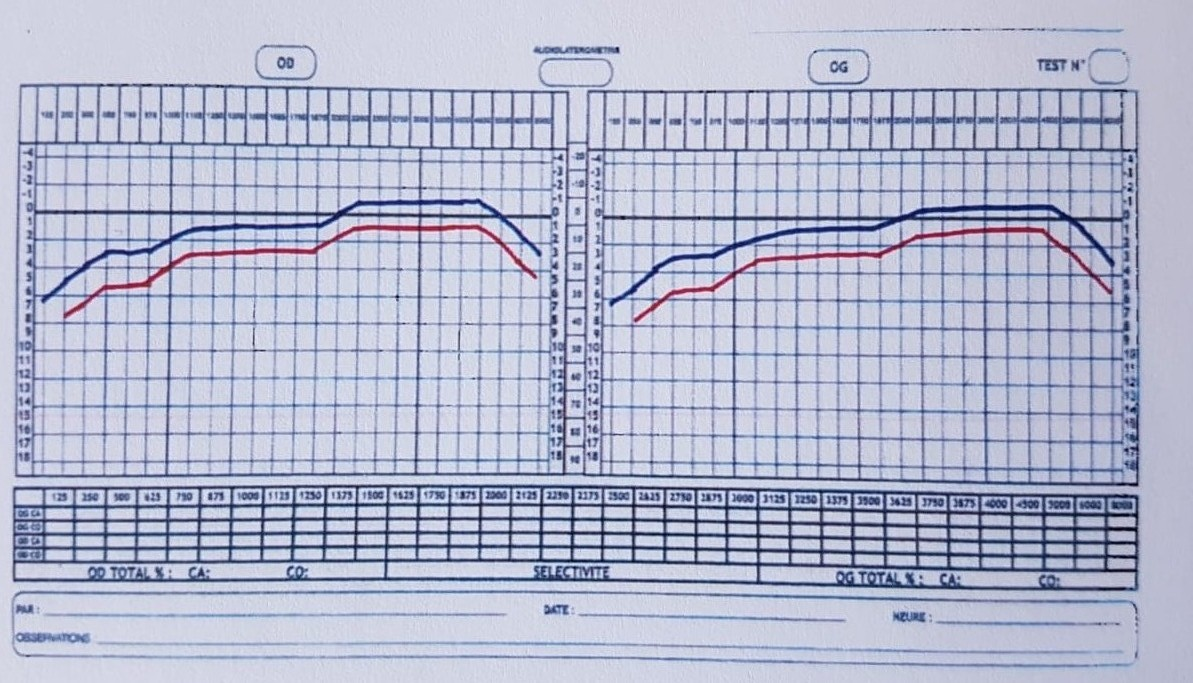
\includegraphics[width=0.7\linewidth]{images/courbeideale.jpg}
	\caption{Courbe idéale}
	\label{fig:courbeideale}
\end{figure}


Sur le plan de la physique pure, elle indique les réponses de l'oreille
lorsque celle-ci fonctionne bien. Elle répond en fait à la courbe
de Wegel dite ``courbe en citron", inversée.\footnote{%
		Voir l'annexe \ref{acoustique} p. \pageref{acoustique}
		 pour cette partie technique.}.

L'acquisition de cette courbe idéale correspond à l'harmonisation
du jeu de deux muscles de l'oreille moyenne. Ce jeu
permet de régler en permanence la pression interne de la vésicule
labyrinthique en faisant intervenir les phénomènes de moindre impédance%
\footnote{Pour la définition de l'impédance voir l'annexe \ref{impedance} 
	p. \pageref{impedance}.}.
 Lorsqu'une onde acoustique rencontre l'interface
séparant deux milieux d'impédances acoustiques différents, une partie
de l'onde est transmise dans l'autre milieu tandis qu'une autre partie
se réfléchit sur l'interface. On cherchera à estimer les quantités
d'énergie acoustique transmises et réfléchies.

Les ondes incidentes ($f_1$) sont transmises pour une part au second
milieu ($f_2$) et pour une autre part, elles sont réfléchies à l'interface
entre le premier et le deuxième milieu jaune ($g_1$) (modifié d'après
Wikipedia, 9 février 2009).
% OGA: pourquoi la parenthèse "modifié d'après Wikipedia"?

L'audiogramme classique donne une courbe déterminée
mais n'indique pas pour autant si l'individu examiné
sait vraiment se servir de cette courbe pour communiquer avec les
autres au travers de son autocontrôle.

Son test permet justement de connaître l'utilisation que sait faire
un sujet de son audition. Un \oe il anatomiquement parfait ne permettra
pas de déceler si le sujet sait s'en servir en visant au fusil ou
en faisant de la peinture. Toutes les nuances de couleurs qui permettent
au peintre de s'exprimer ne sont pas celles que tout un chacun voit\footnote{Conférence, Anvers,1973.}. % OGA: quelle conférence?
% quel orateur? Il faut mettre en biblio.
\enquote{L'écoute est à l'oreille ce que la vision est à
l'\oe il.} % OGA: quel ouvrage, quel page stp?
 Il existe donc \enquote{une dimension de gnosie qui apporte une
donnée complémentaire, [\dots] une dimension d'attention, d'adhésion
qui s'institue dans l'écoute, prise de conscience qui s'imbrique
à l'audition elle-même.}
 
\enquote{Lorsque l'interprétation mentale des informations sensorielles
trans\-mi\-ses par l'oreille est erronée, l'écoute est perturbée.}\autocite{tomatis.com}

Il s'agit de distorsions d'écoute. Cette distorsion est liée au dysfonctionnement
des deux muscles de l'oreille moyenne. Leur rôle est de permettre l'arrivée
harmonieuse du son dans l'oreille interne, puis au cerveau. Car, lorsque
\enquote{le message sensoriel est altéré, le cerveau se protège en déclenchant
des mécanismes d'inhibition de l'écoute.}\marginnote{\footnotesize début de citation mis par OGA. Juste?} Tout enfant peut naître
avec ce potentiel mais celui-ci s'altère parfois avec les difficultés
de la vie. Il se ferme au monde de l'écoute et il introduit des distorsions
pour se défendre contre les agressions du monde extérieur. 

Sur le plan du test d'écoute, on remarquera
alors des distorsions, des manques par rapport à la courbe
idéale qui se trouve sous-jacente dans tout individu. 

% OGA: référence de la citation suivante stp?
\blockquote{La présence d'une \emph{pente ascendante} est nécessaire pour que
l'oreille puisse bloquer les fréquences graves, les atténuer, afin
que la partie proximale de la cochlée soit utilisée, plus particulièrement
dans la zone consacrée au langage. Ceci est spécifique de l'oreille
humaine. Les auditions de certains animaux sont quant aux bandes passantes,
beaucoup plus développées que la nôtre : le dauphin, par exemple,
entend jusqu'à \SI{200000}{\Hz}, certaines chauve-souris,
certains vampires jusqu'à \SI{150000}{\Hz}; un chien entend jusqu'à \SI{45000}{\Hz}. Mais ce sont là des performances qui représentent peu de chose
par rapport à la faculté qu'a l'oreille humaine d'entendre
le langage. Et cette partie d'analyse fine exige qu'elle ne soit pas
gênée par la perception des fréquences graves [\dots] \autocite{Entretien de Tomatis par Auriol}. }

\enquote{\emph{L'oreille a un psychisme\autocite[correct? p.?]{tomatis:loreille}.}} 
L'intégration de l'audio-thérapie et/ou de la musicothérapie a tout son sens dans le contexte ou le milieu psychiatrique. Tomatis, à notre sens, ne pouvait faire meilleure boutade.

De cette phrase, qui peut paraître exagérée,
nous laisse interrogatifs sur la récente parution d'un
article d'une étude franco-américaine scientifique
\autocite{fritz_stradivarius} au sujet des Stradivarius : elle semble ne pas lui donner totalement
tort et même l'atteste d'une autre manière : nous transformons l'écoute
selon nos attentes. Faite avec un protocole d'écoutes en aveugle avec
des violonistes professionnels et en parallèle avec un public (caché
derrière un rideau), cette étude démontre que le mythe de la suprématie
de ces instruments extrêmement chers est tombé au profit d'instruments
neufs. L'étude prouve que le cerveau transforme les informations reçues
selon les attentes que l'on a. Le rôle du cerveau dans notre perceptions\marginnote{\scriptsize Note de la Roque liée à?}
est extrêmement fort et cette étude le prouve scientifiquement
\autocite{lemonde.fr:stradivarius}.
% \footnote{\href{http://www.lemonde.fr/culture/article/2014/04/10/le-stradivarius-detrone-par-les-violons-modernes\_4398681\_3246.html}{LeMonde.fr}.}.

\autocite[p. 43]{roque:lecoute}

\section{Description de la passation du test d'écoute}
\label{passation}

Pour effectuer ce test, un appareil contenant un générateur de fréquences appelé ``\emph{Hearing Test}'', émet des sons purs s'étalant de \SIrange{125}{8000}{\Hz}, d'octave en octave, en passant par les valeurs
\SIlist{1500;3000;6000}{\Hz}, et dont l'intensité, peut varier de 5 en \SI{5}{\dB}, de \SIrange{10}{100}{\dB}. 

Ce test a pour but de déterminer les 4 paramètres suivants : 
\begin{enumerate}
\item seuils;
\item spatialisation;
\item sélectivité;
\item audiolatérométrie.
\end{enumerate}

\subsection{Recherche des seuils}

Il s'agit de rechercher d'une part les seuils d'audibilité
minima : il est demandé au sujet de lever la main du côté
où il entend le son, de lever les deux mains lorsqu'il entend le son
des deux côtés ou lorsqu'il ne peut en déterminer la provenance.

\subsubsection{Deux types de conduction sonore}
Il existe deux types de conduction sonore, l'une \emph{aérienne} et l'autre \emph{osseuse}.

En conduction aérienne, le son pénètre dans le conduit externe de
l'oreille par l'intermédiaire d'écouteurs. Les vibrations du tympan
parviennent à l'oreille interne qui informe le nerf auditif.

En conduction osseuse, le son pénètre à l'aide d'un
vibrateur qui vient exciter la mastoïde. Par l'intermédiaire de la
boîte crânienne, les vibrations informent le nerf auditif.

\subsubsection{Représentation graphique}

\begin{figure}
	\centering
	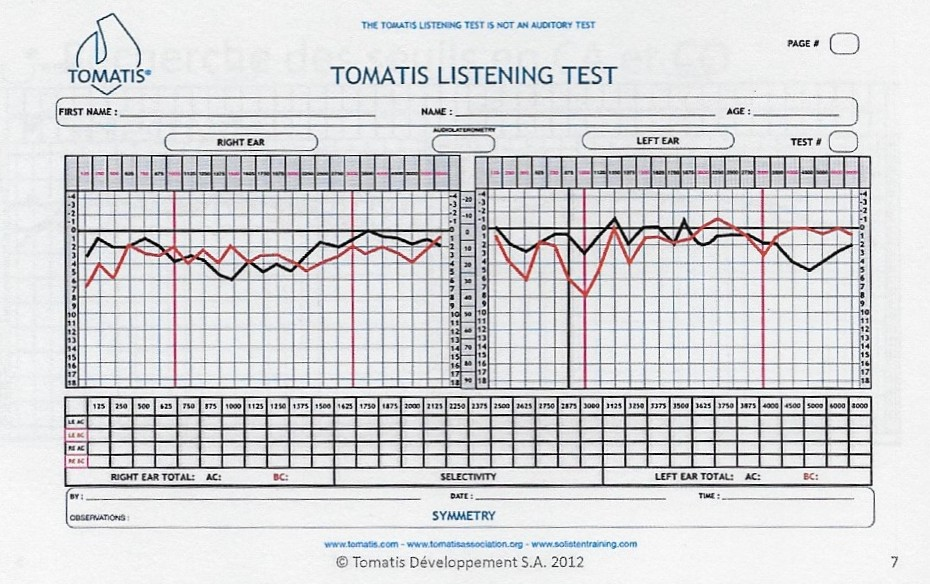
\includegraphics[width=0.7\linewidth]{images/tomatisListeningTest}
	\caption[Graphique du test d'écoute]{Graphique du test d'écoute}
	\label{fig:tomatislisteningtest}
\end{figure}

Les résultats sont consignés sur deux grilles correspondant à la courbe
de l'oreille droite et à celle de l'oreille gauche%
\footnote{Voir fig. \ref{fig:tomatislisteningtest}. Suivant le processus d'observation habituellement appliqué en physiologie,
la place de ces deux diagrammes est inversée, la courbe droite étant
à gauche et la courbe gauche étant à droite.}.

En abscisses, on porte les fréquences de \SIrange{125}{8000}{\Hz}, et en ordonnées,
les intensités en décibels qui se lisent de haut en bas. 

Les seuils reportés sur les graphiques sont reliés entre eux et vont
dessiner deux courbes distinctes\footnote{Tomatis a volontairement décalé les étalonnages des deux courbes (aérienne
	et osseuse) pour pouvoir distinguer les différentes réponses et interpréter
	les distorsions. Lorsque l'écoute est parfaite, les
	courbes aérienne et osseuse se confondent mais pour l'analyse des
	résultats, on a déterminé des courbes parallèles, la courbe aérienne
	devant être au dessus de la courbe osseuse.}: 
\begin{itemize}
	\item la courbe aérienne (CA);
	\item la courbe osseuse (CO) de l'oreille droite et celles de l'oreille gauche.
\end{itemize}



\subsection{\'Etude de la spatialisation}

Lors de la recherche des seuils, on note en même temps le pouvoir
de l'oreille de localiser les sons dans l'espace. On recueille les
confusions ou inversions latérales de sons. Les inversions ou les
confusions de sons sont notées au niveau de chaque fréquence par un
petit trait placé au bas de chacune des grilles. La spatialisation
est un indicateur du degré d'élaboration de la latéralité auditive,
elle donne des repères sur la façon dont le patient intègre les informations
au niveau du cortex, les faisceaux homo et hétéro-latéraux devant
être fonctionnellement différenciés. 

% ici je ferais un nouveau paragraphe
Les erreurs reflètent la confusion
de cette intégration et donnent une indication sur la latence et l'incertitude
dans le traitement de l'information (la manière d'appréhender le
son dans l'espace). Ce peut être la difficulté du sujet à fixer son
écoute, une mauvaise coordination, un manque de confiance en soi ou
une mauvaise organisation des idées.

\subsection{\'Etude de la sélectivité}

La sélectivité est la \textquote{faculté que possède une oreille de percevoir
une variation de fréquences à l'intérieur d'un spectre sonore, et
de situer le sens de cette variation}\autocite{tomatis:loreille}.
Le but est de déceler l'ouverture ou la fermeture de cette sélectivité
auditive. 

% nouveau paragraphe
Pour le faire, on effectue pour chaque oreille, en conduction
aérienne, et à un niveau d'environ \SIlist{40;60}{\dB}, un balayage des
fréquences en partant généralement des aigus. On demande au sujet
d'indiquer si le son perçu est plus aigu, plus grave ou de même hauteur
que le précédent. Les erreurs sont indiquées au niveau des fréquences
mal analysées et le blocage de la sélectivité est indiqué en traits
hachurés à partir de la fréquence la plus grave qui a été marquée
d'un trait. La sélectivité permet de donner des informations sur la
qualité d'écoute avec trois aspects : au niveau linguistique ( conscience
phonémique), cognitif ( fonctions exécutives) et émotionnel ( action
efférente, présence d'anxiété).

\subsection{L'audiolatérométrie}

On recherche la latéralité du patient : droite ou gauche. La dominance
de l'oreille droite comme oreille directrice doit être manifeste.

Ainsi, après la passation du test d\textquoteright écoute, nous nous
trouvons en présence de deux grilles contenant chacune deux courbes,
en général, de deux couleurs différentes complétées par l'indication
des inversions ou confusions de sons, par des données sur la sélectivité
et en même temps par des chiffres qui correspondent à l'épreuve d'audiolatérométrie.

Les résultats du test permettront de faire une comparaison avec la
courbe dite idéale : c'est une courbe ascendante entre 500 et 2000
hz qui correspond à une pente d\textquoteright environ 6 à 18 db/octave,
puis un dôme entre 2000 et 4000 Hz et ensuite une légère descente. 

\paragraph{Les trois zones du test d'écoute : }

Mise en évidence de différentes zones à l\textquoteright intérieur
de chaque diagramme. 

Ces bandes sonores se répartissent en trois zones, des fréquences
graves aux aigues, de la façon suivante :
\begin{itemize}
\item Zone 1 : de 125 à 1000 Hz : les graves, la zone vestibulaire
\item Zone 2 : de 1000 à 3000 Hz : les mediums, la zone du langage
\item Zone 3 : de 3000 à 8000 Hz : les aigus, zone cochléaire
\end{itemize}

\subparagraph*{Pour notre étude, nous allons nous en tenir à celui de la recherche
des seuils : seuil de la courbe aérienne et seuil de l'osseux des
deux oreilles, gauche et droite.}



\paragraph{La première étape : une approche globale : }

Ce sont des comparaisons graphiques des courbes. 

On considère l'allure générale des courbes, on compare leur dessin
: la forme des courbes, l' équilibre, la symétrie ; et on étudie leurs
rapports entre eux : 

courbe aérienne (CA) - courbe osseuse (CO) - rapport entre CA et CO
pour chaque oreille - rapport entre CA et CO d\textquoteright une
oreille à l'autre. si ce rapport est correct, CA est placée au-dessus
de CO sur la grille.
\section{Interprétation du test : }

\subsection{Signification et interprétation psychologique du test : }
\subparagraph{Les deux types de courbes véhiculent chacune des informations spécifiques
sur la posture d'écoute du sujet : }
\begin{itemize}
\item La conduction aérienne : traduit la vie sociale, la manière de communiquer
et de s'extérioriser, permet de préciser la façon dont le sujet\emph{
écoute le monde extérieur} et en particulier l\textquoteright autre,
son interlocuteur, celui qui lui parle. 
\item La conduction osseuse : traduit la vie intérieure, mode de fonctionnement
organique, d'une façon générale : liée aux tensions.C'est la courbe
de l\textquoteright auto-écoute, de l\textquoteright auto-contrôle,
de l'écoute intérieure.
\end{itemize}

\subparagraph{Les courbes donnent des informations selon leur ascendance, leur
continuité et leur similarité oreille droite/ oreille gauche.}
\begin{itemize}
\item Continuité de la courbe : Si une courbe est continue, elle définie
comme harmonieuse et ne comporte pas de pics ou de scotomes (échancrure)  qui laisseraient
supposer l'existence de nombreuse tensions.
\end{itemize}
Situées en CO, ce sont des tensions internes non exprimées : attitude
calme mais très tendue intérieurement.

Situées en CA, ce sont des tensions réelles et exprimées au quotidien
: soit somatisées, soit verbalisées ou soit manifestées sur le plan
affectif (pleurs).

\subparagraph{Les trois zones du test d'écoute : }
\begin{itemize}
\item Zone 1 : de 125 à 1000 Hz : les graves, la zone vestibulaire, élaboration
du schéma corporel, des repères temporo-spatiaux, adresse motrice,
esprit pratique.
\item Zone 2 : de 1000 à 3000 Hz : les mediums, la zone du langage, de la
verbalisation, compréhension, mémorisation, de l'intégration des lois/
des règles, esprit analytique.
\item Zone 3 : de 3000 à 8000 Hz : les aigus, zone cochléaire, de l'énergie,
de l'imagination, de l'expression, motivation, esprit synthétique.
\end{itemize}

\subparagraph{Les trois zones de fréquences du test d'écoute correspondent à des
caractéristiques précises ; et, avec l'allure des courbes, on doit
tenir compte de leurs particularités.}

Lorsqu'une zone du test d'écoute est nettement dominante et semble
traduire une caractéristique de la personnalité, on peut situer un
sujet dans un registre particulier correspondant à son tempérament.

- courbe accentuée dans la zone fréquentielle des graves : tempérament
somatoïde, orienté vers le corps

-courbe accentuée dans la zone fréquentielle des médiums : tempérament
paranoïde, attaché à la logique, la règle, le raisonnement 

-courbe accentuée dans la zone fréquentielle des aigus : tempérament
schizoïde, reflétant une recherche de créativité. 

\subparagraph{Signification des diagrammes droite et gauche : }

Selon Tomatis, l'oreille gauche correspond à \textquoteright l'affectivité,
au passé, à la mère, et la droite, au père, au devenir.

Pour cette étude, nous nous en tiendrons à la première étape. La deuxième est aussi passionnante mais nous aurez demandé encore beaucoup de temps pour l'analyser à fond. Néanmoins, nous aimerions la mentionner.

\subparagraph{La deuxième étape : l'approche analytique du nombres d'erreurs en
spatialisation et en sélectivité.}


Ce sujet est très complexe. Néanmoins, nous pouvons signaler que : 
\begin{itemize}
\item lorsqu'il y a une sélectivité fermée, on peut parler de fermeture
à l'univers environnant.
\item Lorsqu'il y a des déficiences d'analyse dans une zone située dans
les graves, en général, la puissance sélective des aigus est inexistante.
Le sujet ne peut utiliser les bandes situées au dessus de la zone
non sélective. Celle ci est une sorte de barrière qui cantonne le
sujet dans la zone des graves. 
\item Certains scotomes ( pertes) situés dans la zone des graves constituent
une deuxième barrière qui empêche l'individu d'aller au delà de cette
zone. Le sujet n'utilisera pas la plage sonore correspondant aux aigus. 
\end{itemize}

La chaîne parlée est faite de milliers de phonèmes que l'on doit savoir
distinguer pour que le mot atteigne sa véritable signification. Le
test de sélectivité est justement fait pour que l'on reconnaisse les
possibilités auditives du sujet à l\textquoteright égard d'un son
pur qui est une simplification énorme par rapport à un mot. Un son
\char`\"{}pur\char`\"{} comme son nom l'indique est un son dépouillé
de toute ambiguité qu'il doit être facile de distinguer d'un autre
et de situer par rapport à cet autre. Si donc l\textquoteright individu
ne peut pas opérer cette opération sélective entre sons purs, il est
difficile qu'il puisse distinguer les subtilités, les infinies variations,
les multiples couleurs que revêt un mot à l'intérieur d'une phrase.
L'oreille humaine a des possibilités d'analyse exceptionnelle. Elle
peut percevoir à 1000 hertz une différence de 3 Hertz ; elle peut
aussi déceler le sens de cette variation, reconnaître s'il s'agit
d'un son de 997 hertz , ou de 1000 hertz , tout en le situant dans
l\textquoteright échelle des fréquences. En conséquence, elle peut
facilement distinguer la différence qui existe d'un octave à l'autre,
c'est-à-dire entre les deux sons purs que l'on envoie dans l\textquoteright oreille
du sujet.

\subparagraph{La latéralité auditive : }

Il existe deux types de latéralité auditive lorsqu'on évoque l'écoute:

-quelle est l'oreille que le sujet utilise pour écouter l'autre ?
( oreille droite ou oreille gauche tendue)

-quelle est l'oreille qu'il utilise pour contrôler son propre langage?
( écoute de soi)
\begin{itemize}
\item Lorsque le patient est latéralisé à gauche, il met son interlocuteur
à distance et sa vitesse d'assimilation des informations est lente.
\end{itemize}
Elle occasionne beaucoup de fatigue. Son débit verbal est ralenti,
il n'a pas de fluidité. Il peut chanter faux sans s'en rendre compte.
Il est souvent dévoré par son émotivité, submergé par les souvenirs
et privilégie les représentations du passé.
\begin{itemize}
\item Lorsque le patient est droitier d'oreille, il se projette plus facilement
dans l'avenir, il va droit au but, sans perdre de temps. Par contre,
s'il est hyperdroitier, il se révélera souvent agressif, par absence
de sensibilité. Un hypergaucher, quant à lui, perdra constamment ses
moyens.
\end{itemize}
Par conséquent, il serait de bon aloi d'intégrer un équilibre droite/gauche,
avec dominance du côté droit sur le gauche. Cela permet de vivre en
envisageant l'avenir, de prendre des décisions qui font simultanément
appel à notre sensibilité individuelle et à notre souplesse d'adaptation
aux réalités extérieures.

Selon Tomatis, il est possible de lire et d'interpréter sur un test
d'écoute l'image du corps intégrée, depuis les pieds (fréquences graves)
jusqu'à la tête (fréquences aigues). En faisant un tableau des fréquences,
on remarque que les sons les plus graves (16 à 20 périodes) correspondent
à la hauteur du corps de l'homme. Chaque longueur d'onde touche, informe
une partie du corps, des pieds jusqu'à la tête, les sons graves correspondant
à la partie basse, et les sons aigus (ondes courtes) à la partie haute.
Réparties de cette façon, les fréquences du langage sont donc adaptées
au corps humain afin de pouvoir l'informer en totalité. En matière
de langage, les hommes sculptent leur corps en fonction des sons qu'ils
émettent. La zone du langage est importante parce qu'elle représente
en fait l'image du corps.

Tomatis relève ``\emph{ l'alliage indissociable du corps et du psychisme,
visible et lisible, résultat de l'écoute de sons.''}\footnote{\emph{Extrait de l'entretien Tomatis réalisé par Auriol, Anvers 1973}}

C'est un sujet qui serait intéressant d'approfondir et qui pourrait
donner des réflexions intéressantes à faire avec la musicothérapie.
